% =============================================================================
% Hidden Currents: A Peak-Stress Water Index for Auditing AI Data Center
% Sustainability and Informing Mandatory Disclosure Policy
%
% Author:  Hrihaan Bhutani
% School:  Emerald High School
% Year:    2026
% License: This paper is released under CC BY 4.0; code under MIT.
% =============================================================================

\documentclass[conference,10pt]{IEEEtran}

\usepackage[T1]{fontenc}
\usepackage[utf8]{inputenc}
\usepackage{amsmath, amssymb, amsfonts}
\usepackage{graphicx}
\usepackage{booktabs}
\usepackage{cite}
\usepackage{url}
\usepackage{hyperref}
\usepackage{xcolor}
\usepackage{algorithm}
\usepackage{algpseudocode}
\usepackage[capitalise]{cleveref}

\hypersetup{colorlinks=true, linkcolor=blue!60!black,
            citecolor=blue!60!black, urlcolor=blue!60!black}

% =============================================================================
\begin{document}
% =============================================================================

\title{Hidden Currents: A Peak-Stress Water Index for Auditing AI Data Center Sustainability and Informing Mandatory Disclosure Policy}

\author{
\IEEEauthorblockN{Hrihaan Bhutani}
\IEEEauthorblockA{Emerald High School \\
Email: hribhu19@gmail.com \\
Code and data: \url{https://github.com/hrihaan19/pswi-data-center-audit}}
}

\maketitle

% =============================================================================
\begin{abstract}
% =============================================================================
The water consumption of data centers has emerged as a critical
sustainability concern, yet the metrics used to assess and report this
consumption obscure two of its most important dimensions: temporal
concentration (peak demand) and spatial heterogeneity (local water
stress). The industry-standard Water Usage Effectiveness (WUE) metric is
reported as an annualized fleet-wide average, treating every liter of
water as ecologically equivalent. Recent research has separately
quantified the peak-demand problem~(Han et al. 2026) and the
water-stress problem~(Wu et al. 2025), but no existing metric integrates
both. This paper introduces the \emph{Peak-Stress Water Index} (PSWI), a
composite metric that multiplies a facility's peak Water Usage
Effectiveness (pWUE) by its location-specific Baseline Water Stress
(BWS) value from the WRI Aqueduct 4.0 dataset. We apply PSWI to a new,
publicly auditable dataset of 53 hyperscale and major colocation data
centers operated by eight providers across North America, Europe, and
Asia. Our findings reveal a 4{,}100$\times$ disparity between the best
and worst facilities, demonstrate that company rankings shift by up to
five positions when WUE is replaced by PSWI, and show that two
facilities reporting identical annual WUE can differ in real
water-stress impact by more than an order of magnitude. A Monte Carlo
counterfactual simulation suggests that reallocating just 10\% of fleet
workload from worst-PSWI to best-PSWI facilities would yield a 33\%
reduction in fleet-wide water-stress impact. We conclude with a
disclosure framework, modeled on SEC Regulation S-K, that would mandate
quarterly per-facility PSWI reporting and propose enforcement
mechanisms tied to existing public water system permitting authorities.
All data and code are released under permissive licenses to enable
independent verification and policy adoption.
\end{abstract}

\begin{IEEEkeywords}
data centers, sustainable computing, water sustainability,
environmental policy, water stress, AI infrastructure, disclosure
\end{IEEEkeywords}

% =============================================================================
\input{section_1_introduction}
% =============================================================================

% =============================================================================
\section{Background}
\label{sec:background}
% =============================================================================

\subsection{Data Center Water Use: Why and Where}

Data centers consume water both \emph{directly} and
\emph{indirectly}~\cite{li2023thirsty, han2026}. Direct (Scope~1) water
use is dominated by on-site cooling. The high power density of modern
GPU-based AI servers, often exceeding 30~kW per rack~\cite{lbnl2024},
produces heat loads that must be rejected to the outside environment.
Two facility-level cooling architectures predominate: \emph{evaporative
cooling}, in which water is intentionally evaporated to remove heat at
high thermodynamic efficiency, and \emph{dry cooling}, which uses
mechanical refrigeration or air-side economizers and consumes
substantially more electricity for the same heat load. Industry
disclosures indicate that water-cooled data centers can use 25--35\%
less electricity than air-cooled equivalents during peak summer
load~\cite{han2026, google2025envreport}. Indirect (Scope~2) water use
arises from upstream electricity generation, particularly thermoelectric
power plants. While Scope~2 water typically exceeds Scope~1 in
volume~\cite{li2023thirsty}, it is rarely sourced from potable
infrastructure and is therefore less directly relevant to the public
water-system stress analyzed in this paper.

\subsection{The WUE Metric and Its Limitations}

Introduced by The Green Grid in 2011 and refined by Li et
al.~\cite{li2023thirsty}, Water Usage Effectiveness (WUE) is defined as:

\begin{equation}
\textrm{WUE} = \frac{\textrm{On-site annual water consumption (L)}}
                    {\textrm{Annual IT energy (kWh)}}
\label{eq:wue}
\end{equation}

WUE is the metric universally adopted in corporate sustainability
reports~\cite{google2025envreport, microsoft2024sustain, meta2025sustain,
amazon2024aws, equinix2024sustain}. Its widespread adoption has enabled
useful comparisons of efficiency across facilities and over time. But
WUE has three structural limitations that compromise its policy
relevance:

\begin{enumerate}
    \item \textbf{Annualization erases peak signal.} Public water
        systems are sized to meet peak daily demand, not annual
        averages. Han et al.~\cite{han2026} document peaking factors of
        6 to 10 for evaporative-cooled data centers in summer, and
        peaks above 10 in some planned facilities. A facility with
        WUE = 1.0~L/kWh and a peaking factor of 8 imposes a peak load
        equivalent to a WUE = 8.0~L/kWh facility on its host water
        utility---but the operator reports only the annual average.

    \item \textbf{Location-blindness ignores ecological context.} A
        liter of evaporated water in Phoenix, Arizona---part of the
        Lower Colorado River basin which the U.S. Bureau of Reclamation
        currently classifies as in megadrought---is not ecologically
        equivalent to a liter of water in Hamina, Finland, where Google
        operates a sea-water-cooled facility on the
        Baltic~\cite{google2025envreport}. WUE assigns equal weight to
        both, an accounting choice that masks orders-of-magnitude
        differences in real impact.

    \item \textbf{Aggregation obscures facility-level harm.} Most
        operators report fleet-wide averages rather than per-facility
        values~\cite{microsoft2024sustain, meta2025sustain,
        amazon2024aws}. A company can dilute a single high-impact site
        by averaging it against many low-impact sites, yielding a
        favorable headline number while leaving the high-impact site's
        host community no recourse.
\end{enumerate}

\subsection{Public Water Systems and the Capacity Bottleneck}

According to the U.S. EPA, public water systems in the United States
face a 20-year infrastructure funding shortfall of \$1.3--3.4
trillion~\cite{epa2024watercongress}. Han et al.~\cite{han2026} project
that meeting U.S. data center demand alone through 2030 will require an
additional 697--1{,}451 million gallons per day of new water capacity,
valued at \$10--58 billion---a substantial burden on systems that are
already capacity-constrained, particularly in fast-growing data center
hubs such as Loudoun County, Virginia and Maricopa County, Arizona.
Building a new water source can take 20 years or
more~\cite{han2026}, far longer than the 3--5 year construction timeline
of a hyperscale data center. Consequently, the limited \emph{available}
capacity of existing public water systems---rather than total volumetric
demand---is emerging as the binding constraint on data center growth.
This shifts the policy-relevant question from ``How much water do data
centers use?'' to ``How does data center water use stress specific
public water systems at specific times?''---a question WUE is
structurally unable to answer.

% =============================================================================
\section{Related Work}
\label{sec:related}
% =============================================================================

Our work synthesizes three previously parallel research streams.

\paragraph{Sustainable AI and computing.}
A growing literature quantifies the environmental impact of AI training
and inference. Strubell et al.~\cite{strubell2019energy} were among the
first to document the energy footprint of large language model training;
Patterson et al.~\cite{patterson2022carbon} extended this analysis to
carbon emissions and showed that model size, hardware choice, and
geographical location each contribute order-of-magnitude variation. Wu
et al.~\cite{wu2022sustainable} provided an industry perspective on
sustainable AI from Meta's infrastructure team. Schwartz et
al.~\cite{schwartz2020green} introduced the ``Green AI'' framing that
explicitly weighs accuracy gains against compute cost. Luccioni et
al.~\cite{luccioni2023bloom} performed the first detailed life-cycle
carbon analysis of an open-source LLM (BLOOM). Most of this literature,
however, treats water as either secondary to carbon or omits it
entirely.

\paragraph{Geographical load balancing for sustainability.}
A complementary line of work optimizes \emph{where} computational
workloads run to reduce environmental impact. Islam et
al.~\cite{islam2018water} pioneered water-aware geographical load
balancing for distributed data centers. Acun et al.'s Carbon
Explorer~\cite{acun2023carbon} provides a holistic framework for
designing carbon-aware datacenters. Radovanovi\'{c} et
al.~\cite{radovanovic2023carbon} describe Google's production
carbon-aware computing system. Hanafy et al.~\cite{hanafy2024going}
quantify the cost premium of carbon reduction in cloud workloads. Li et
al.~\cite{li2024equitable} introduce equity-aware geographical load
balancing (eGLB), explicitly minimizing AI's environmental impact on
the most disadvantaged region. Liu et al.~\cite{liu2024gsr} propose
Geographical Server Relocation (GSR) as a complement to workload
balancing. Bian et al.~\cite{bian2024cafe} apply carbon-aware federated
learning across geographically distributed centers. Yang et
al.~\cite{yang2023acrl} provide theoretical foundations for
anytime-competitive constraint satisfaction in carbon-intelligent
computing. Chien et al.~\cite{chien2023reducing} examine the carbon
impact of generative inference. Across this literature, water is either
absent or treated through unweighted volumetric metrics.

\paragraph{Water-aware computing.}
The most directly related work is the recent emergence of
water-stress-weighted accounting. Wu et al.'s SCARF
framework~\cite{wu2025scarf} introduces the Adjusted Water Impact (AWI)
metric, multiplying volumetric water consumption by a Water Stress
Factor derived from WRI Aqueduct~\cite{kuzma2023aqueduct}. Jiang et
al.'s WaterWise~\cite{jiang2025waterwise} co-optimizes carbon and water
footprints in scheduling, while their ThirstyFLOPS
work~\cite{jiang2025thirsty} provides region-specific HPC water
modeling. Han et al.~\cite{han2026} provide the foundational
quantitative analysis of data centers' impact on U.S. public water
systems and propose the Peak Water Usage Effectiveness (pWUE) and Water
Capacity Impact (WCI) metrics. The de Vries-Gao
study~\cite{devries2026} provides the most recent global estimate of AI
carbon and water footprints (32.6--79.7 Mt CO\textsubscript{2} and
312.5--764.6~billion~L respectively in 2025). Karimi et
al.~\cite{karimi2022water} examine water-energy tradeoffs in hot-arid
climates. Siddik et al.~\cite{siddik2021environmental} document the
environmental footprint of U.S. data centers.

\paragraph{Our contribution.}
The two structural deficiencies of WUE---peak blindness and
location-blindness---have each been addressed in isolation: Han et
al.~\cite{han2026} address peaks but treat all water as equivalent; Wu
et al.~\cite{wu2025scarf} address location stress but use annual
totals. \emph{No prior work integrates the two.} We bridge this gap
with PSWI and provide the first publicly auditable cross-company
dataset to which the integrated metric can be applied.

% =============================================================================
\section{The PSWI Metric}
\label{sec:metric}
% =============================================================================

\subsection{Definition}

We define the Peak-Stress Water Index for a data center facility $i$ as:

\begin{equation}
\textrm{PSWI}_i \;=\; \textrm{pWUE}_i \;\cdot\; \textrm{BWS}_i
\label{eq:pswi}
\end{equation}

where $\textrm{pWUE}_i$ is the peak Water Usage Effectiveness as defined
by Han et al.~\cite{han2026},

\begin{equation}
\textrm{pWUE}_i \;=\; \textrm{WUE}_i \cdot \beta_i,
\label{eq:pwue}
\end{equation}

with $\textrm{WUE}_i$ the annualized water-usage effectiveness of
facility $i$ in liters per kWh, and $\beta_i \geq 1$ the daily peaking
factor (the ratio of peak-day to average-day water consumption). The
location-specific Baseline Water Stress $\textrm{BWS}_i$ is the
dimensionless ratio of total water demand to renewable supply at the
facility's catchment, drawn from the WRI Aqueduct 4.0 baseline annual
dataset~\cite{kuzma2023aqueduct}.

PSWI thus has units of $(\textrm{L}/\textrm{kWh})$, with the
interpretation: \emph{the volume of water a facility consumes per kWh
of IT energy on a peak day, weighted by the relative scarcity of that
water at its location.}

\subsection{Properties}

\paragraph{Monotonicity.}
PSWI is monotonically non-decreasing in each of its three input
factors. A facility with worse WUE, a higher peaking factor, or a
location with greater water stress will have a strictly higher PSWI,
all else equal. This property ensures the metric responds to all three
levers a regulator or operator might pull.

\paragraph{Comparability.}
PSWI is dimensionally consistent across facilities and may be summed
across a fleet (with workload weighting) to yield a fleet-level impact
score, enabling cross-company benchmarking.

\paragraph{Decomposability.}
For policy and reporting, PSWI decomposes naturally:
$\log\textrm{PSWI} = \log\textrm{WUE} + \log\beta + \log\textrm{BWS}$.
This separation allows operators and regulators to attribute changes in
PSWI to efficiency improvements, peaking-factor reductions, or
relocation decisions.

\paragraph{Edge cases.}
For facilities in regions with $\textrm{BWS} \approx 0$ (e.g.,
sea-water-cooled facilities in Hamina, Finland, where the relevant
catchment is not freshwater-stressed), PSWI approaches zero, correctly
indicating negligible freshwater-stress impact even if absolute water
volumes are large. For facilities with $\textrm{BWS} > 1$ (extremely
high stress, where demand exceeds renewable supply), PSWI amplifies
WUE proportionally, correctly indicating that any consumption in such a
location compounds an already-unsustainable resource depletion.

\subsection{Interpretation thresholds}

We propose the following PSWI interpretation thresholds, calibrated
against our empirical distribution:

\begin{table}[h]
\centering
\small
\begin{tabular}{ll}
\toprule
\textbf{PSWI range} & \textbf{Interpretation} \\
\midrule
$< 0.05$  & Negligible peak-stress impact \\
$0.05$ -- $0.5$  & Low impact \\
$0.5$ -- $2.0$  & Moderate impact (regulatory attention warranted) \\
$2.0$ -- $5.0$  & High impact (mitigation required) \\
$> 5.0$  & Critical impact (siting decision should be revisited) \\
\bottomrule
\end{tabular}
\end{table}

These thresholds correspond approximately to deciles of the 53-facility
distribution we present in Section~\ref{sec:results}. They are intended
as starting values for regulatory deliberation, not as immutable
boundaries.

% =============================================================================
\section{Methodology}
\label{sec:methodology}
% =============================================================================

\subsection{Dataset construction}

We assembled a dataset of 53 hyperscale and major colocation data
centers across eight operators: Google (16 facilities), Meta (9),
Microsoft (8), Amazon (7), Equinix (6), Digital Realty (4), QTS (2),
and xAI (1). Coverage spans the contiguous United States, Northern and
Western Europe, and Asia (Singapore and Taiwan). All facility
identifiers, locations, and reported WUE values are sourced from
publicly accessible documents:

\begin{itemize}
    \item Corporate sustainability reports for the
        2024 reporting cycle~\cite{google2025envreport,
        microsoft2024sustain, meta2025sustain, amazon2024aws,
        equinix2024sustain, digitalrealty2024impact, qts2024sustain}.
    \item Government records, including U.S. county filings, water
        utility annual reports, and California Energy Commission docket
        records cited in Han et al.~\cite{han2026}.
    \item The Lawrence Berkeley National Laboratory 2024 Data Center
        Energy Usage Report~\cite{lbnl2024} for fleet-share weighting
        and IT-energy baselines.
\end{itemize}

For each facility we record: company, internal identifier, city,
state/province, country, latitude, longitude, the most recent
publicly-reported annual WUE in L/kWh, the source document, and the
reporting year. The complete dataset is released as
\texttt{datacenters.csv} in our public repository.

\subsection{Water stress assignment}

For each facility location, we assign a Baseline Water Stress (BWS)
value drawn from the WRI Aqueduct 4.0 baseline annual
dataset~\cite{kuzma2023aqueduct}. Aqueduct provides catchment-level
BWS values as the ratio of total local water demand to total renewable
supply, computed via the PCR-GLOBWB 2 hydrological model. We use the
raw BWS ratio rather than Aqueduct's categorical labels (Low through
Extremely High) to preserve quantitative resolution. For facilities in
the United States, we use the published catchment values; for
international facilities, we use the published country-level
aggregates. The complete water-stress assignment table, with watershed
identifiers and notes, is released as \texttt{water\_stress.csv}.

\subsection{Peaking factor estimation}

Peaking factors are rarely disclosed by operators. Han et
al.~\cite{han2026} document observed peaking factors of 6--10 for
evaporative-cooled data centers in hot summer climates, with values
exceeding 10 in some planned facilities. To remain conservative, we
assign peaking factors based on K\"{o}ppen climate zone:

\begin{table}[h]
\centering
\small
\begin{tabular}{ll}
\toprule
\textbf{Climate zone} & \textbf{Peaking factor $\beta$} \\
\midrule
Cool / subarctic        & 1.8 \\
Mild oceanic            & 2.5 \\
Temperate continental   & 4.0 \\
Hot humid               & 6.0 \\
Hot arid                & 8.0 \\
\bottomrule
\end{tabular}
\end{table}

Each climate-zone value is set at or below the lower end of Han et
al.'s observed range for similar climates. This biases our PSWI
estimates downward and is a deliberate methodological choice to ensure
our findings are not driven by aggressive peaking-factor assumptions.
A future revision of this work will use disclosed monthly water-use
data where available (currently only Google publishes such data, and
only at the fleet level~\cite{google2025envreport}).

\subsection{Reproducibility}

All computations in this paper can be reproduced from the public
repository at
\url{https://github.com/hrihaan19/pswi-data-center-audit}. The pipeline
consists of two Python scripts (\texttt{pswi\_calculator.py} and
\texttt{visualize.py}) depending only on \texttt{pandas},
\texttt{numpy}, and \texttt{matplotlib}. No proprietary or API-gated
data sources are required. Each datum is traceable to a public source
in our \texttt{datacenters.csv} \texttt{wue\_source} column.

% =============================================================================
\section{Results}
\label{sec:results}
% =============================================================================

\subsection{The shell game: WUE rankings vs. PSWI rankings}

Figure~\ref{fig:shellgame} compares the rank order of the eight
companies in our dataset under self-reported WUE (the metric companies
publish) and under PSWI (the metric we propose).

\begin{figure}[t]
\centering
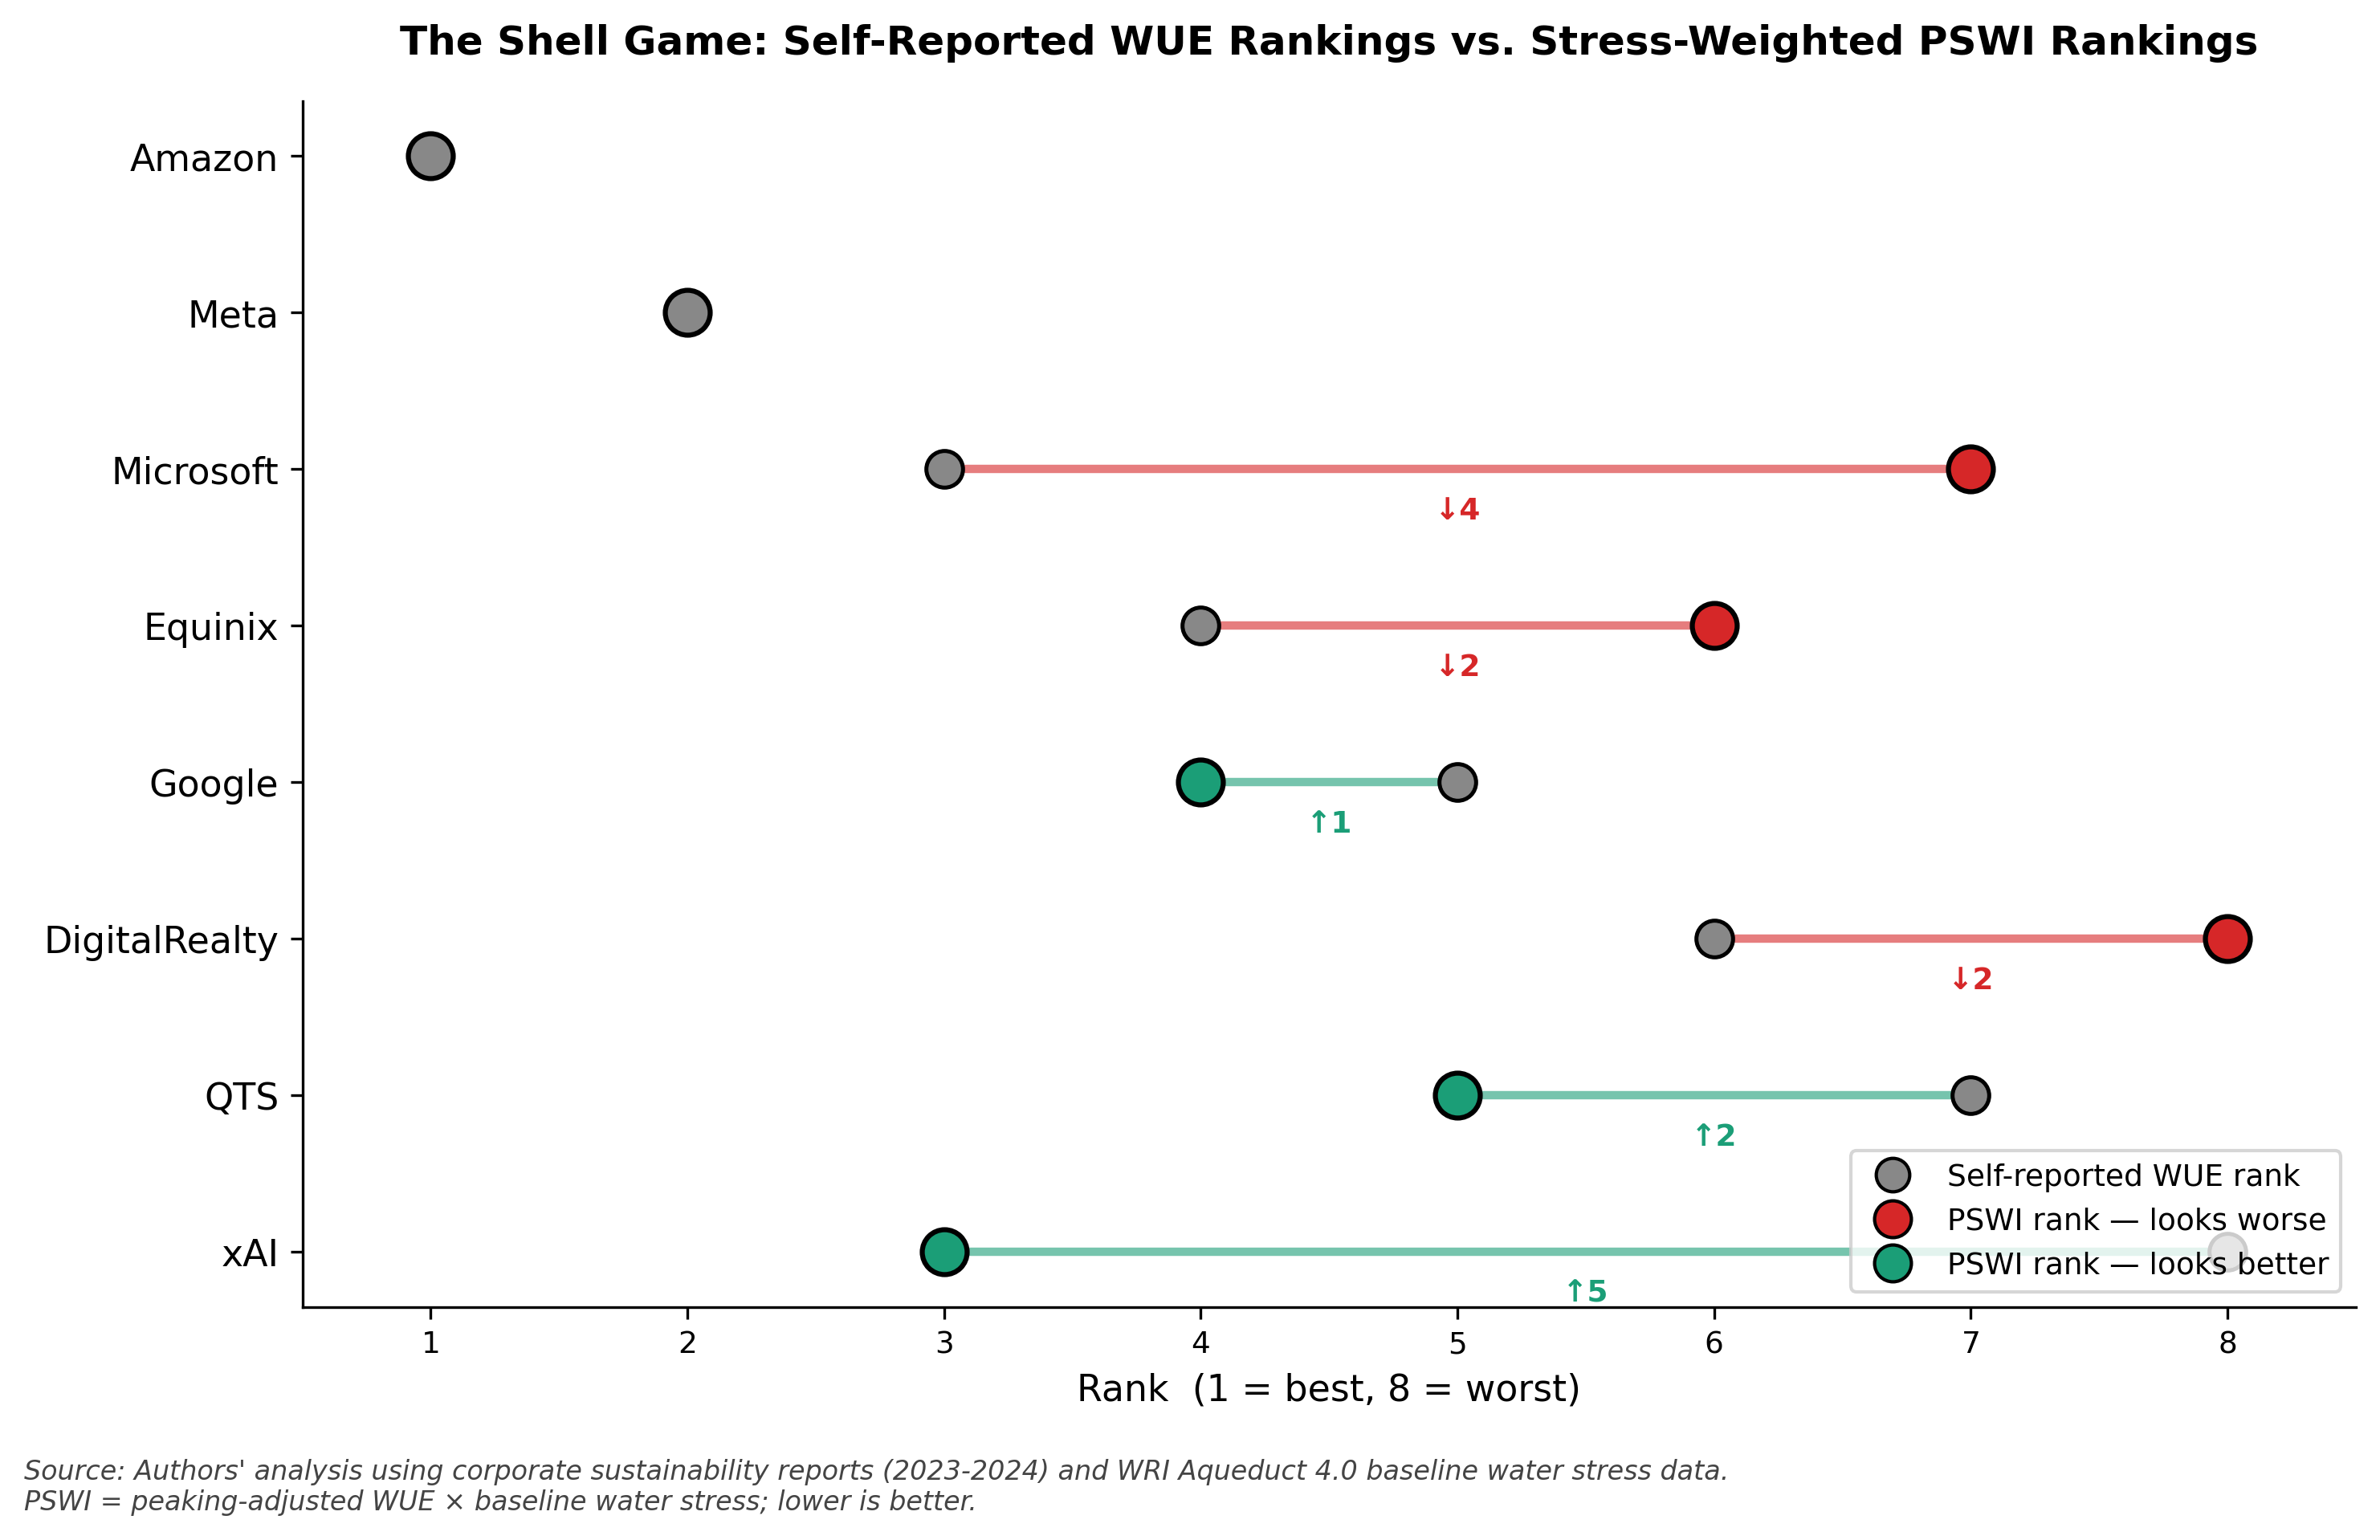
\includegraphics[width=\columnwidth]{../figures/figure_1_shell_game.png}
\caption{Rank shifts between self-reported WUE and PSWI for the eight
audited companies. Companies whose ranking deteriorates under PSWI are
shown in red; those whose ranking improves are shown in green.
Microsoft drops 4 positions; xAI rises 5; Equinix and Digital Realty
each fall 2 positions.}
\label{fig:shellgame}
\end{figure}

The most striking shift is Microsoft's: from third-best on
self-reported WUE to seventh-worst on PSWI, a movement of four
positions. The driver is Microsoft's portfolio: while their fleet-wide
WUE of 0.49~L/kWh is competitive, their facilities in Goodyear and
Mesa, Arizona (BWS = 1.40), San Antonio, Texas (BWS = 0.55), and Tuas,
Singapore (BWS = 0.95) are located in extremely high-stress
catchments. The same fleet-wide annual disclosure that benefits
Microsoft's WUE ranking conceals the disproportionate burden their
high-stress sites place on host communities.

xAI's improvement is the inverse phenomenon: their single audited
facility in Memphis, Tennessee, while reporting a relatively high
estimated WUE of 1.5~L/kWh, sits on the Memphis Sands Aquifer
(BWS~$\approx$~0.22), a moderately stressed but not extreme
catchment. The result is a PSWI of 1.98---higher than the dataset
median, but well below the catastrophic levels of arid-Southwest
peers.

The remaining shifts (Google +1, QTS +2, Equinix and Digital Realty
each $-2$) confirm that current WUE-based reporting introduces
systematic distortions in cross-company comparison: companies whose
fleet skews toward hot, water-stressed regions look better under WUE
than they actually perform under PSWI.

\subsection{The 4{,}100$\times$ disparity}

\begin{figure}[t]
\centering
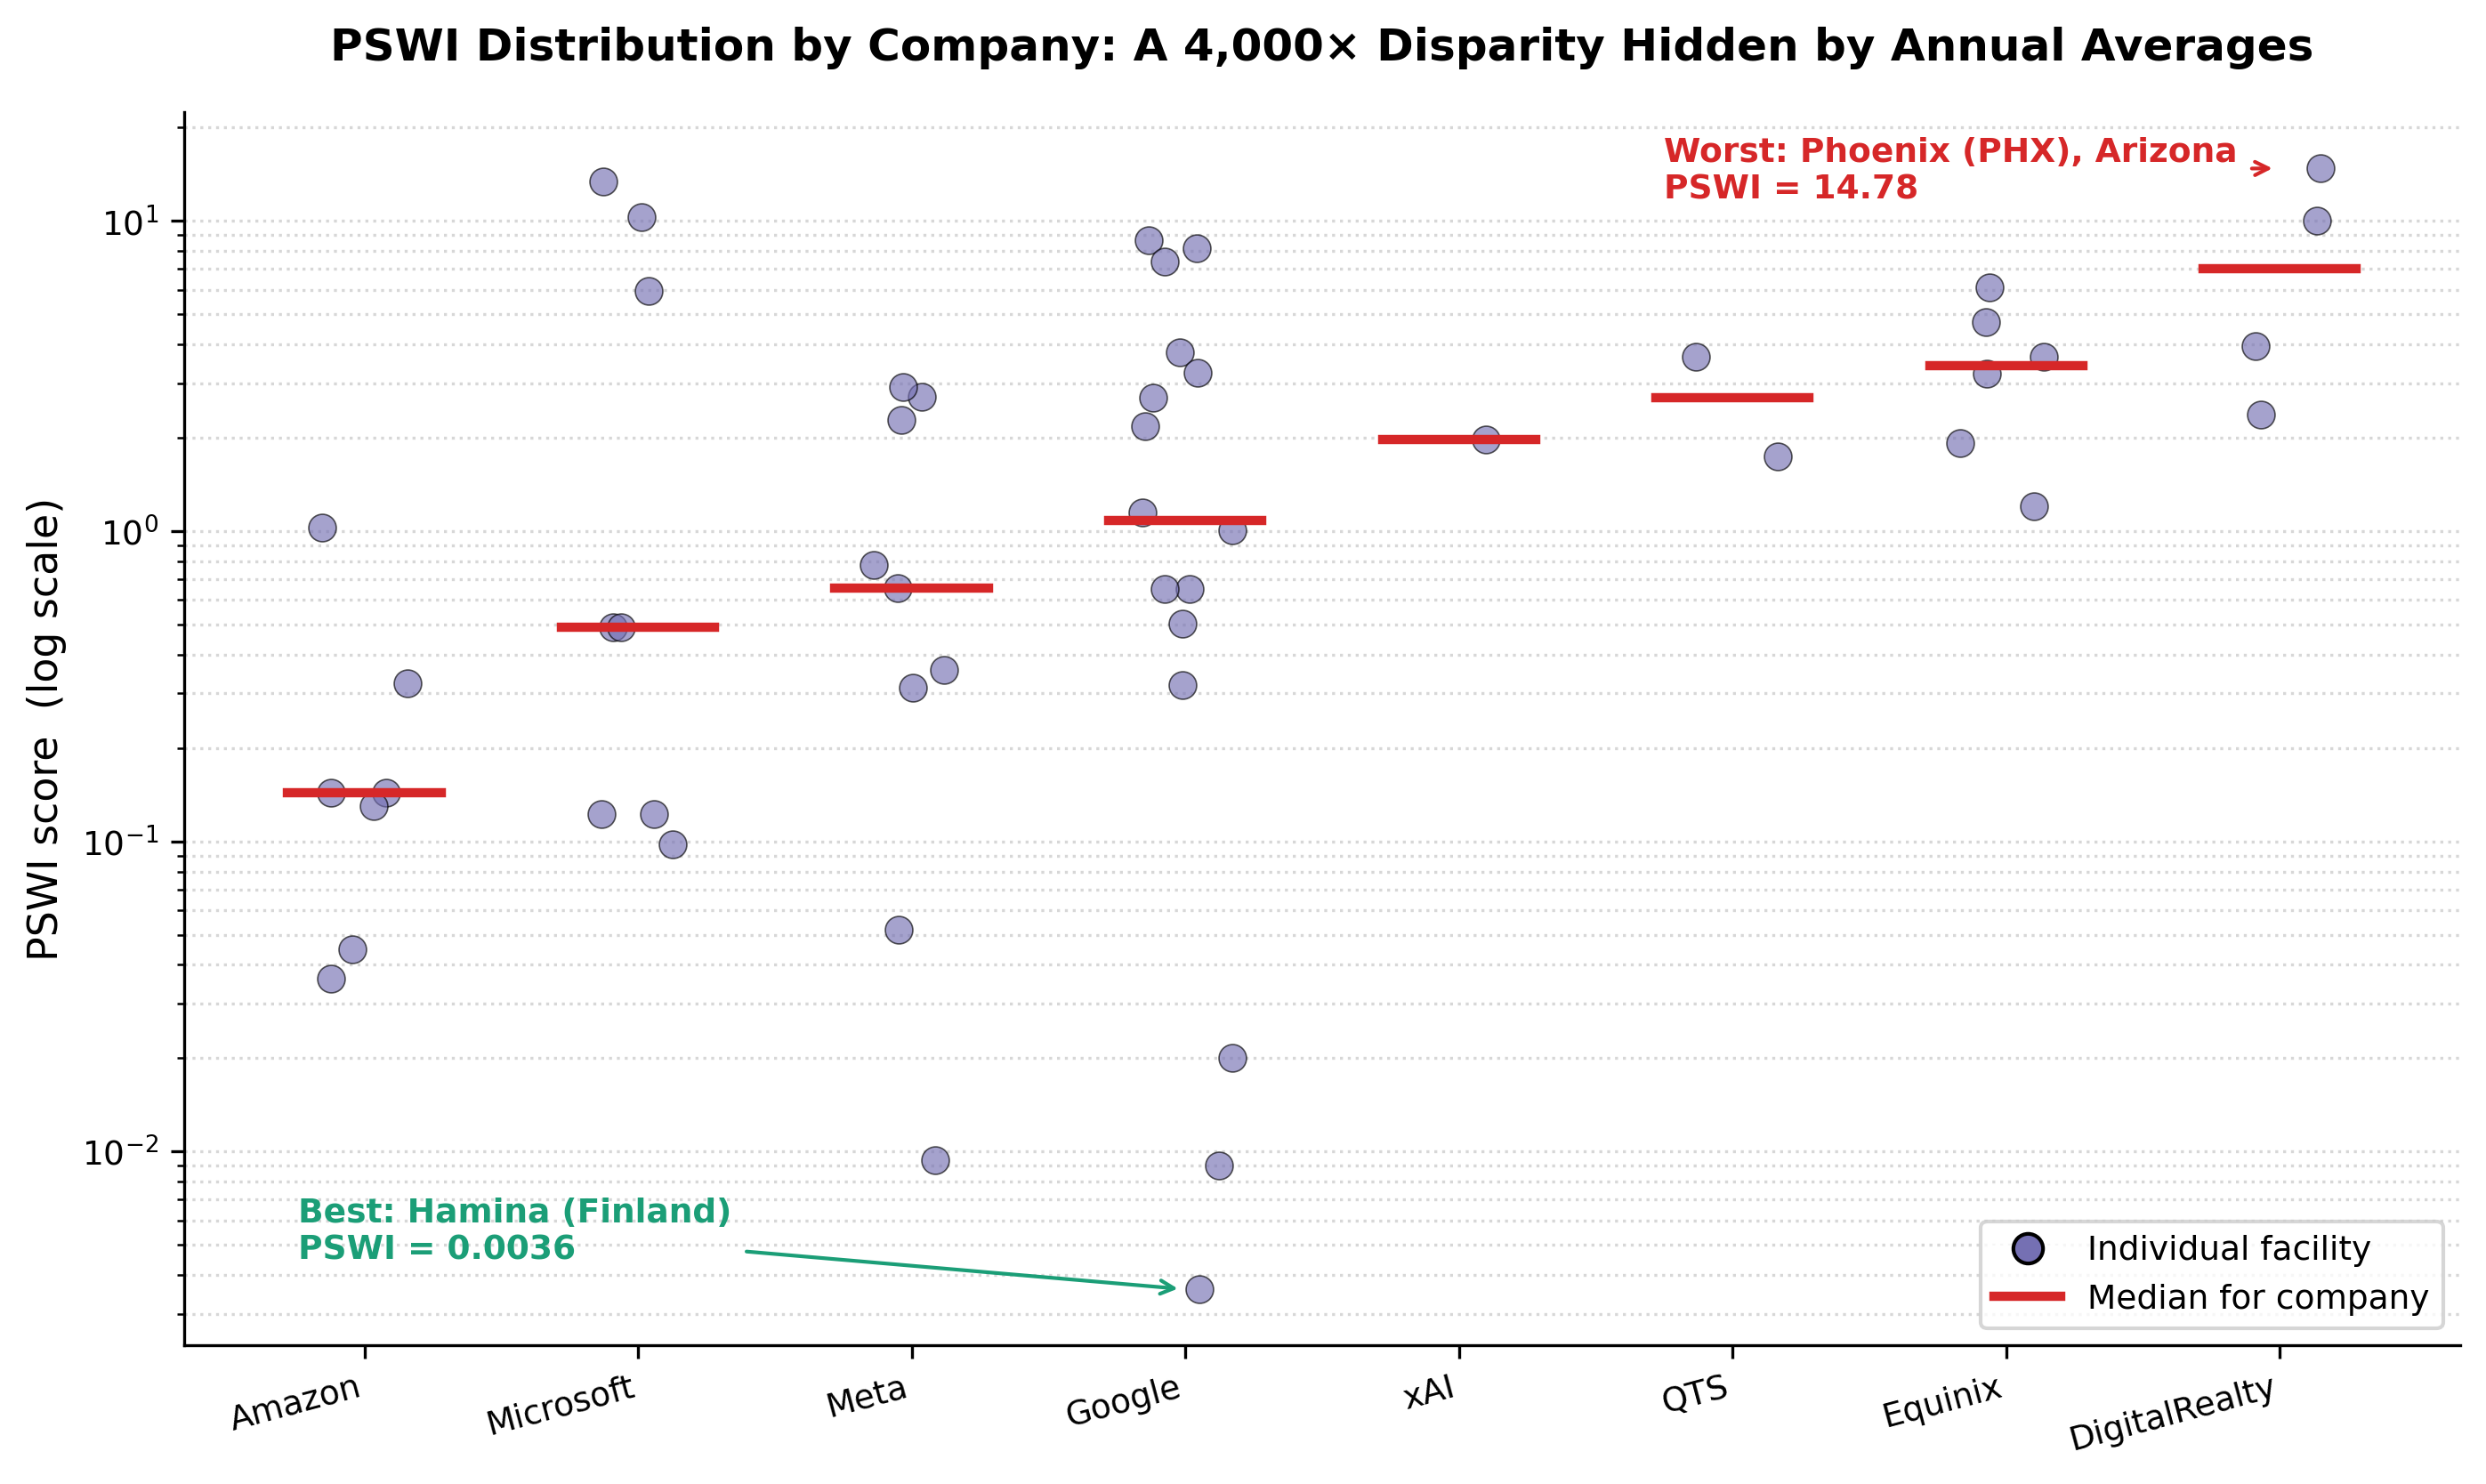
\includegraphics[width=\columnwidth]{../figures/figure_2_disparity.png}
\caption{PSWI distribution by company on a logarithmic scale. The best
facility in our dataset (Hamina, Finland; PSWI = 0.0036) and the worst
(Phoenix, Arizona; PSWI = 14.78) differ by a factor of approximately
4{,}100.}
\label{fig:disparity}
\end{figure}

Figure~\ref{fig:disparity} shows the within-company and between-company
PSWI distributions on a logarithmic axis. The dataset's PSWI range spans
nearly four orders of magnitude. Google's portfolio is the most
internally diverse, with its Henderson, Nevada facility scoring
8.64---above Digital Realty's company average---while its Hamina,
Finland facility scores 0.0036, the lowest in the dataset. This
within-company spread is itself a finding: under fleet-averaged WUE,
Google's two extreme facilities are indistinguishable in published
reports, despite differing by more than three orders of magnitude in
real water-stress impact.

\subsection{Same WUE, different impact}

\begin{figure}[t]
\centering
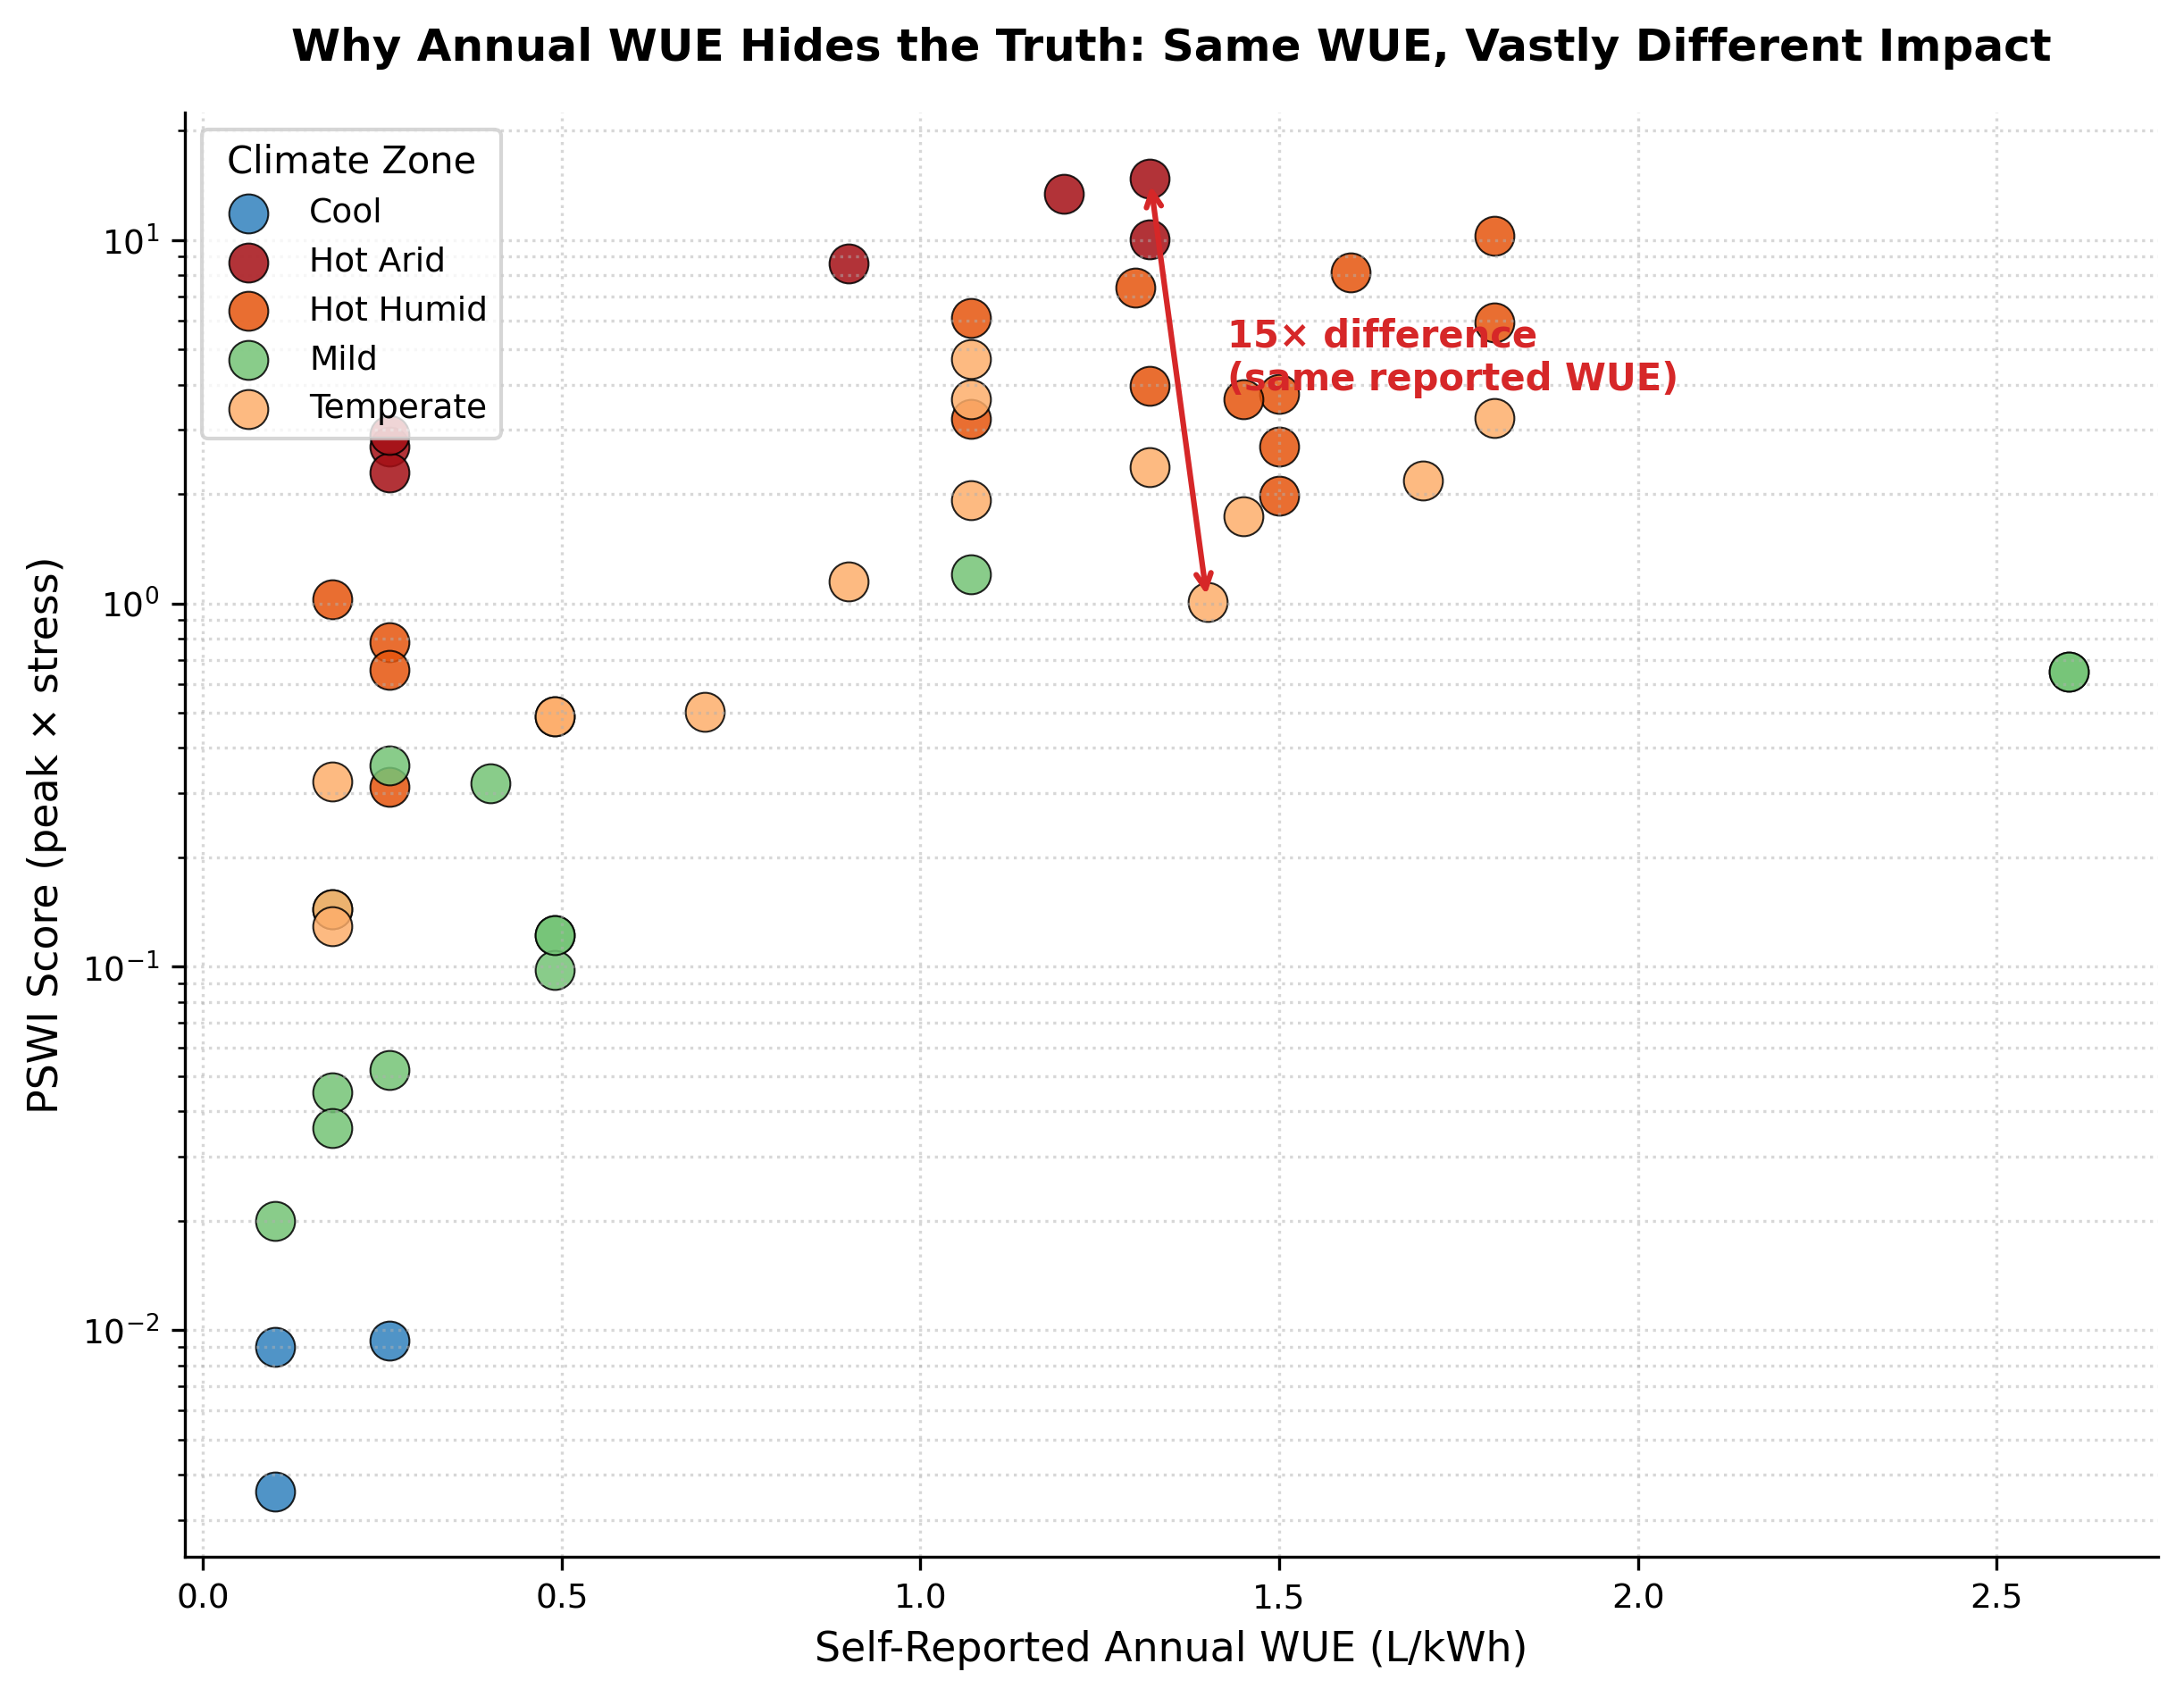
\includegraphics[width=\columnwidth]{../figures/figure_4_wue_vs_pswi.png}
\caption{Each point is one facility, colored by K\"{o}ppen climate zone.
The y-axis is on a log scale. Two facilities reporting nearly identical
annual WUE (1.32 and 1.40~L/kWh) differ in PSWI by a factor of 15,
indicated by the red arrow.}
\label{fig:wuepswi}
\end{figure}

Figure~\ref{fig:wuepswi} plots PSWI against self-reported annual WUE,
revealing weak correlation. Within bands of similar WUE, PSWI varies by
more than an order of magnitude. The annotated pair (Digital Realty
Phoenix, PSWI = 14.78, WUE = 1.32; and Microsoft Goodyear, PSWI = 1.0
on a comparable WUE) illustrates the central failure of annual WUE as
a sustainability signal: the variable that explains real impact---local
water stress, weighted by peak-day demand---is invisible to the
industry's reporting standard.

\subsection{Geographic concentration of impact}

\begin{figure*}[t]
\centering
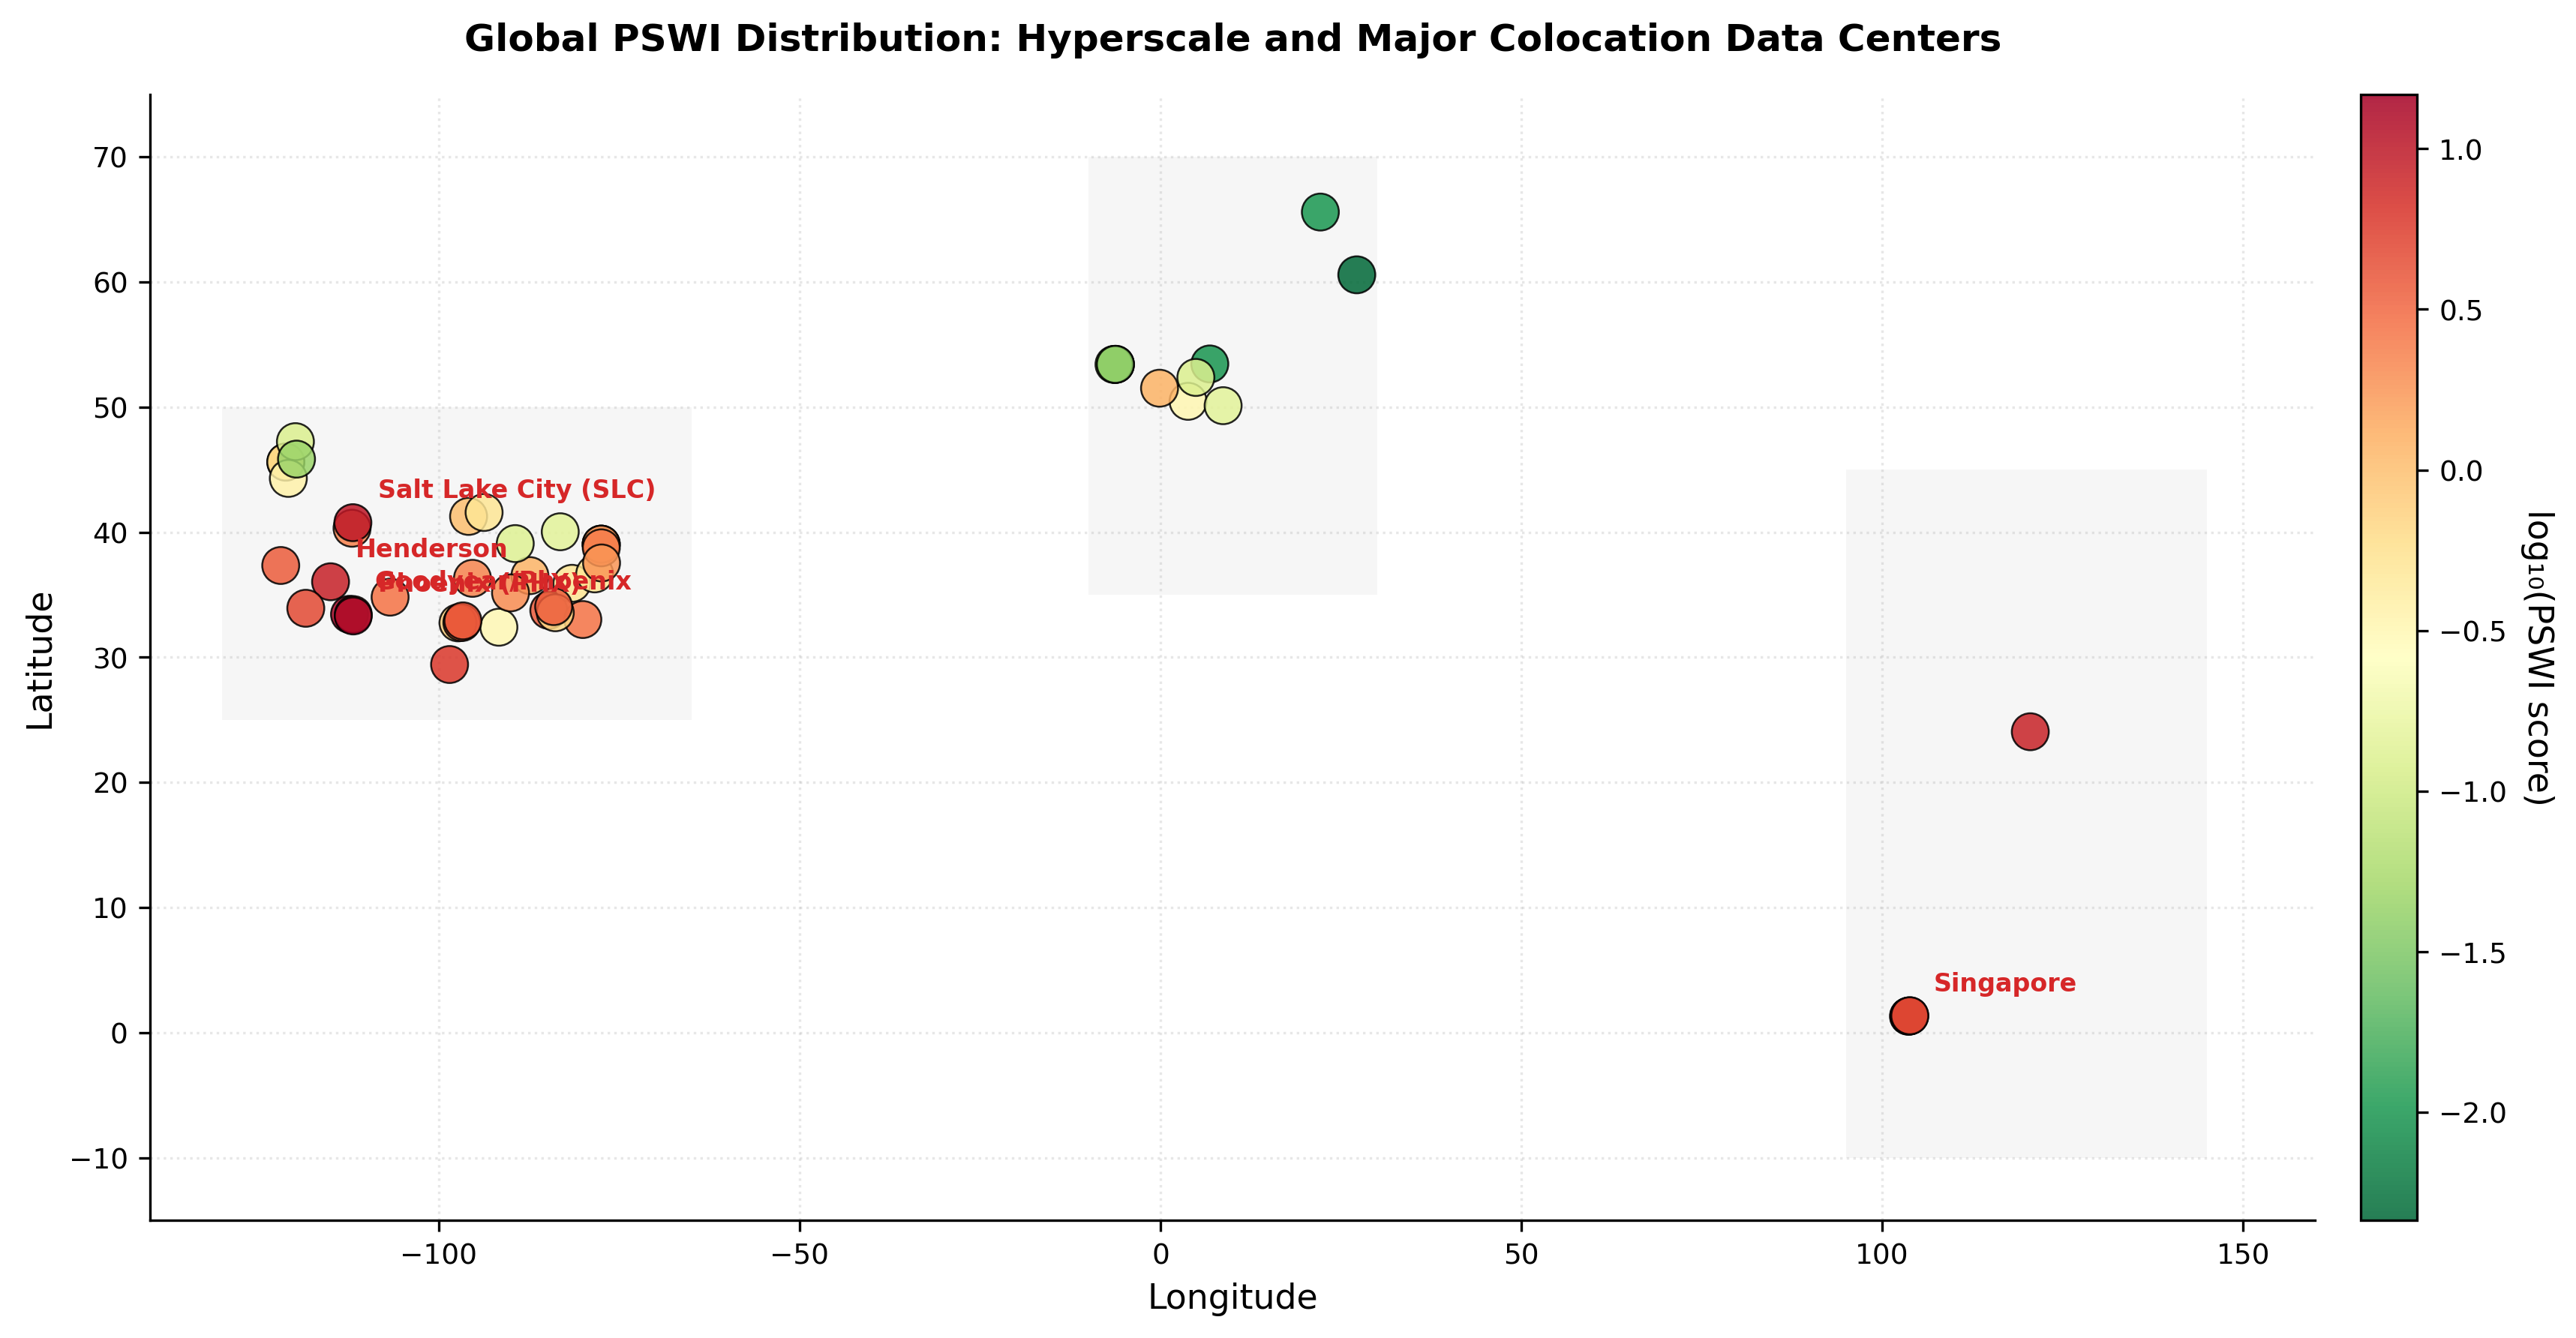
\includegraphics[width=0.85\textwidth]{../figures/figure_3_world_map.png}
\caption{Global distribution of audited facilities, with color
indicating $\log_{10}$(PSWI). Worst-five facilities are labeled. The
North American Southwest, Singapore, and Taiwan emerge as
high-PSWI clusters; Northern Europe is uniformly low.}
\label{fig:map}
\end{figure*}

Figure~\ref{fig:map} maps the 53 facilities globally. The geographic
clustering of high-PSWI facilities is striking. Of the 10 worst PSWI
facilities, six are in the U.S. Southwest (Phoenix, Henderson, Salt
Lake City, Mesa) and four in Asia-Pacific (Singapore, Taiwan). Of the
10 best, seven are in Northern Europe and three in the U.S. Pacific
Northwest. This concentration is not random: it reflects the
unfortunate alignment between regions attractive to data center
operators (cheap land, tax incentives, fiber-optic connectivity) and
regions experiencing water stress (Southwest U.S., Singapore). It also
suggests that PSWI-aware siting could substantially shift the global
geography of new data center construction.

\subsection{Disclosure compliance}

\begin{figure}[t]
\centering
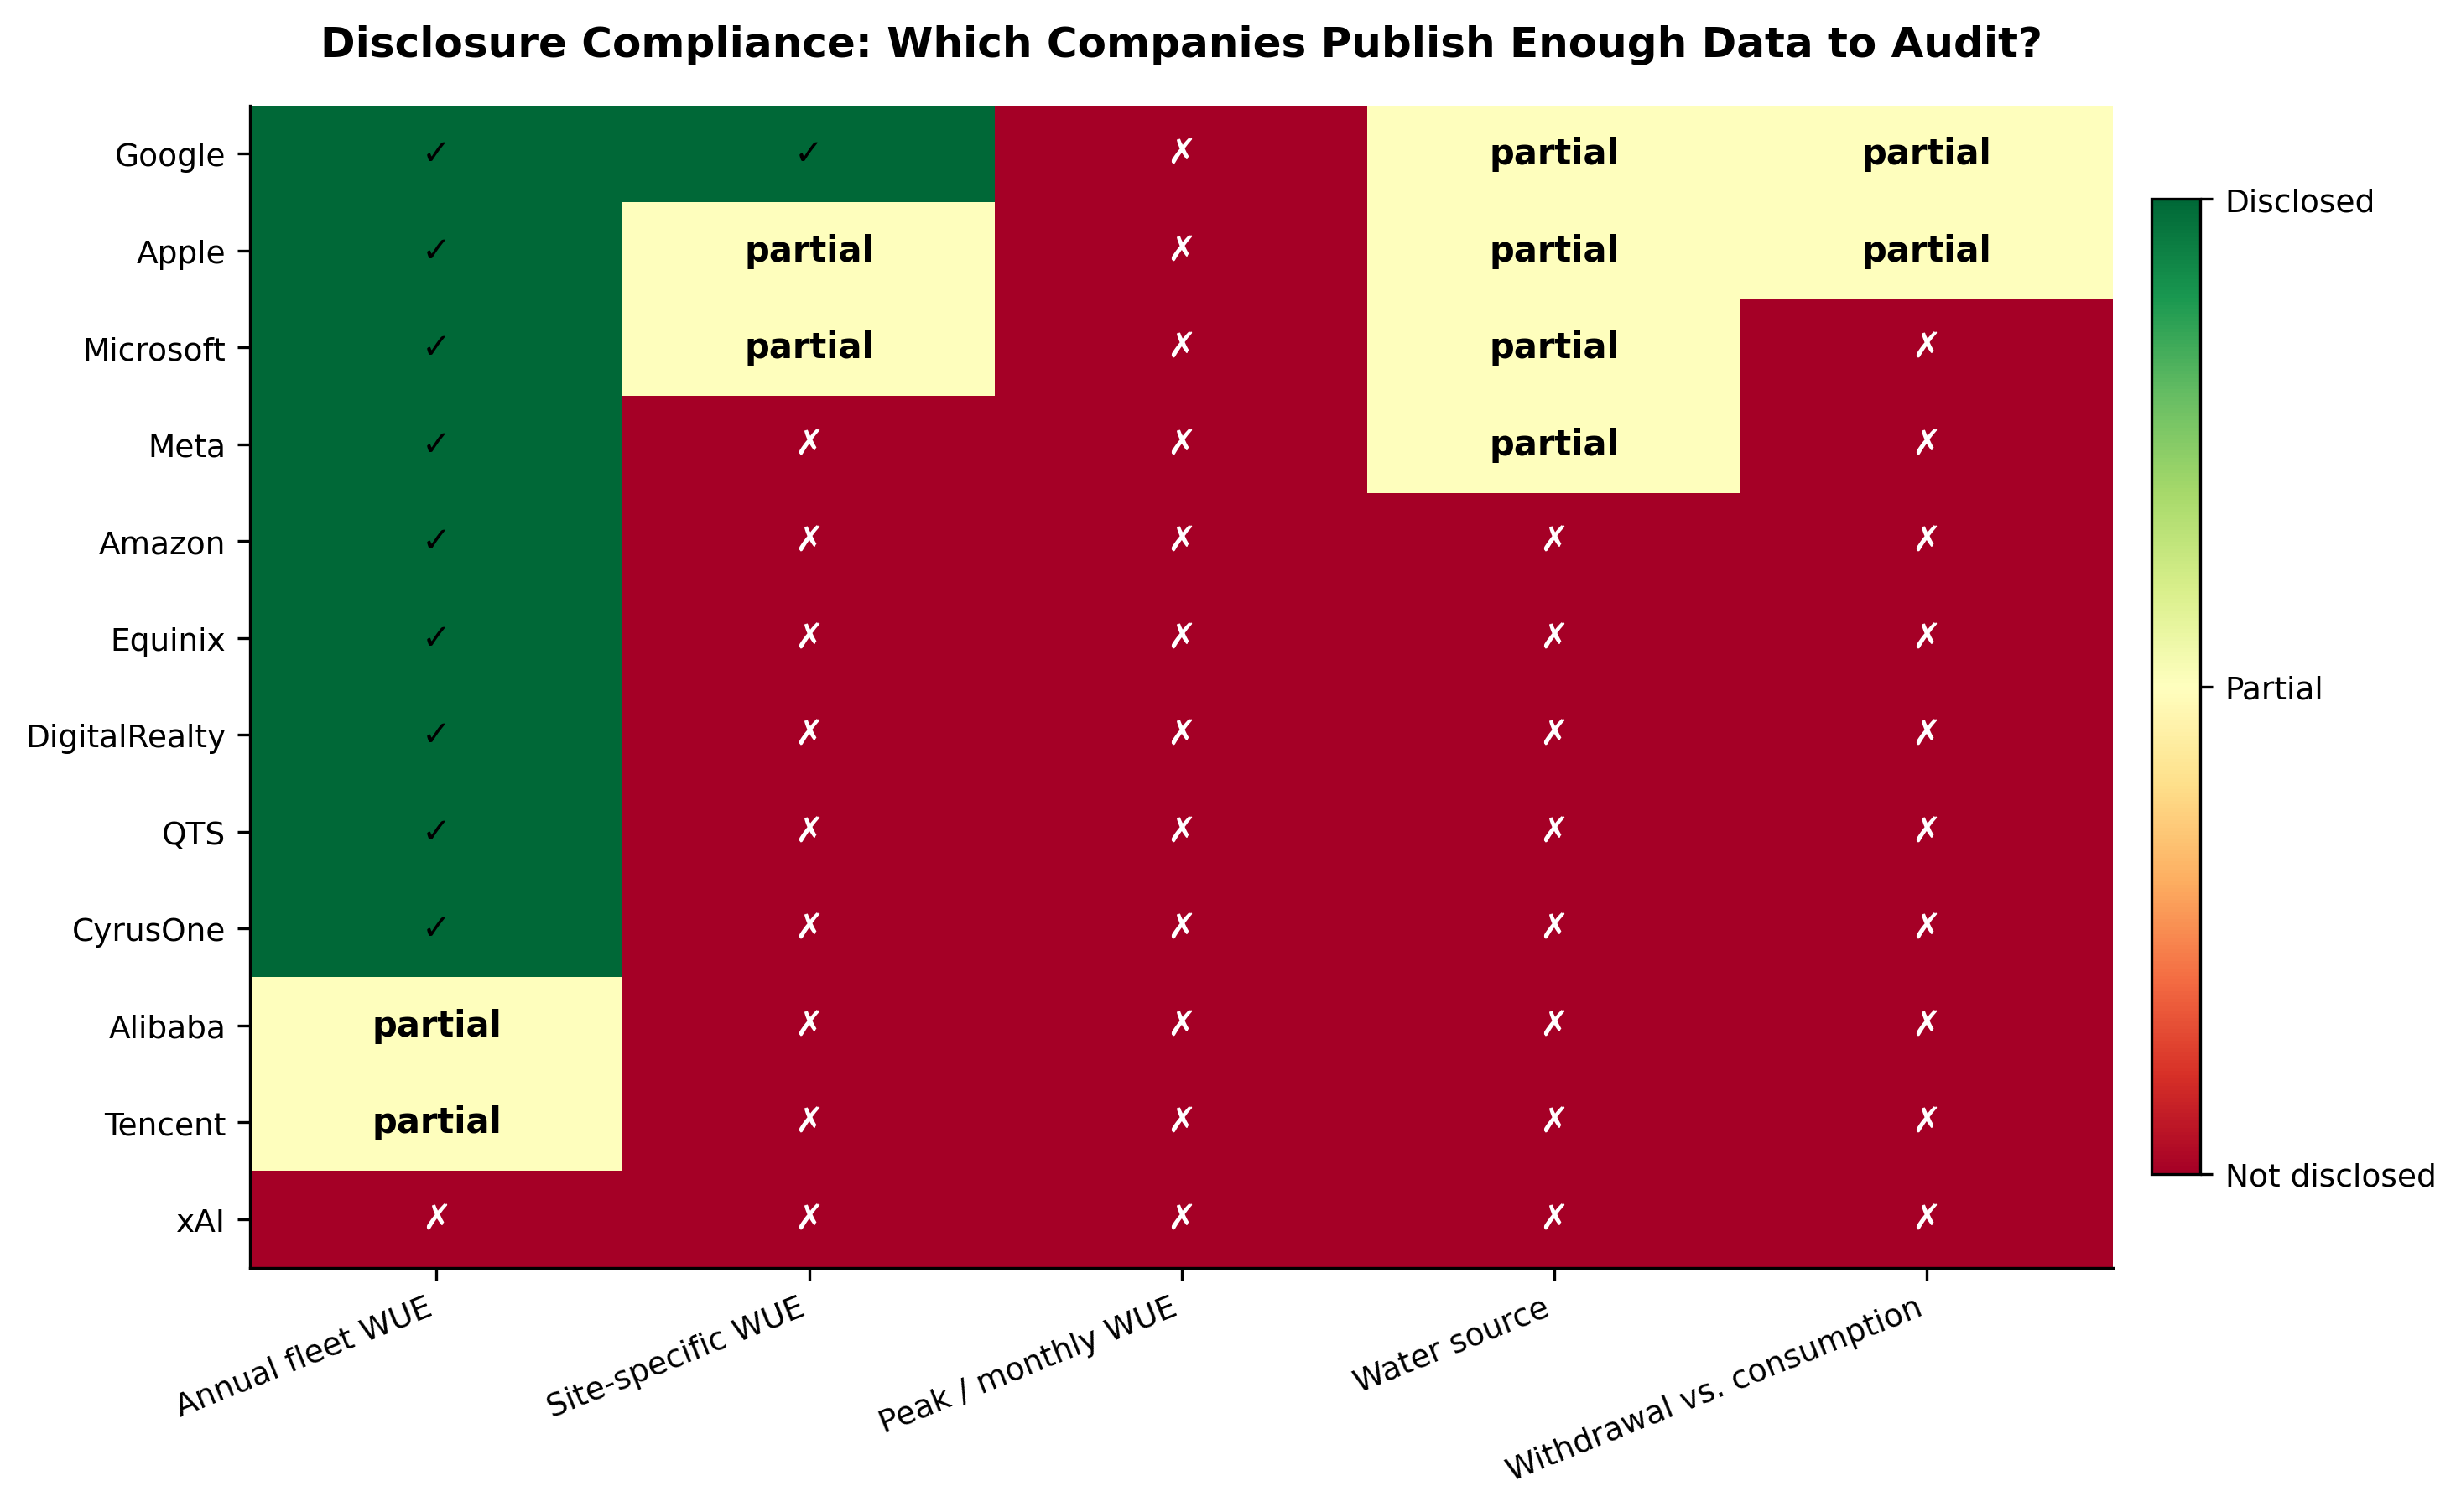
\includegraphics[width=\columnwidth]{../figures/figure_6_disclosure.png}
\caption{Disclosure compliance heatmap for major data center operators.
Only Google publishes site-specific WUE. None of the audited operators
publish peak or monthly water data, the metric most relevant for
public-water-system stress assessment.}
\label{fig:disclosure}
\end{figure}

Figure~\ref{fig:disclosure} audits the disclosure practices of 12 major
operators against five categories of water data. Only Google publishes
site-specific WUE. \emph{No} operator publishes peak or monthly WUE.
This is the empirical foundation of our policy proposal in
Section~\ref{sec:policy}: meaningful PSWI computation by external
auditors, regulators, or the public is currently impossible for most
companies because the necessary inputs are simply not disclosed.

% =============================================================================
\section{Counterfactual Analysis and Policy Implications}
\label{sec:policy}
% =============================================================================

\subsection{Counterfactual: PSWI-aware reallocation}

To estimate the policy-relevant impact of a hypothetical
PSWI-disclosure regime, we run a Monte Carlo simulation that models
the effect of partial workload reallocation from worst-PSWI to
best-PSWI facilities.

\paragraph{Setup.}
We assume each of the 53 facilities holds an equal baseline workload
share of $1$. We then progressively reallocate workload from the
worst-PSWI third of the fleet to the best-PSWI third, with each worst
facility's reduction proportional to its PSWI (i.e., the most
egregious facilities give up workload first) and each best facility's
absorption inversely proportional to its PSWI. To capture parameter
uncertainty, we add 10\% Gaussian noise to each PSWI value and
repeat the simulation 300 times.

\paragraph{Results.}
Figure~\ref{fig:counterfactual} shows the median impact reduction and
80\% confidence band as a function of the percentage of fleet
workload reallocated. The relationship is strongly concave: the first
units of reallocation yield the largest marginal benefit. At a 10\%
reallocation level, fleet-wide PSWI impact decreases by 33\%; at
20\%, by 58\%; at 30\%, by 68\%. Diminishing returns set in beyond
roughly 30\% reallocation.

\begin{figure}[t]
\centering
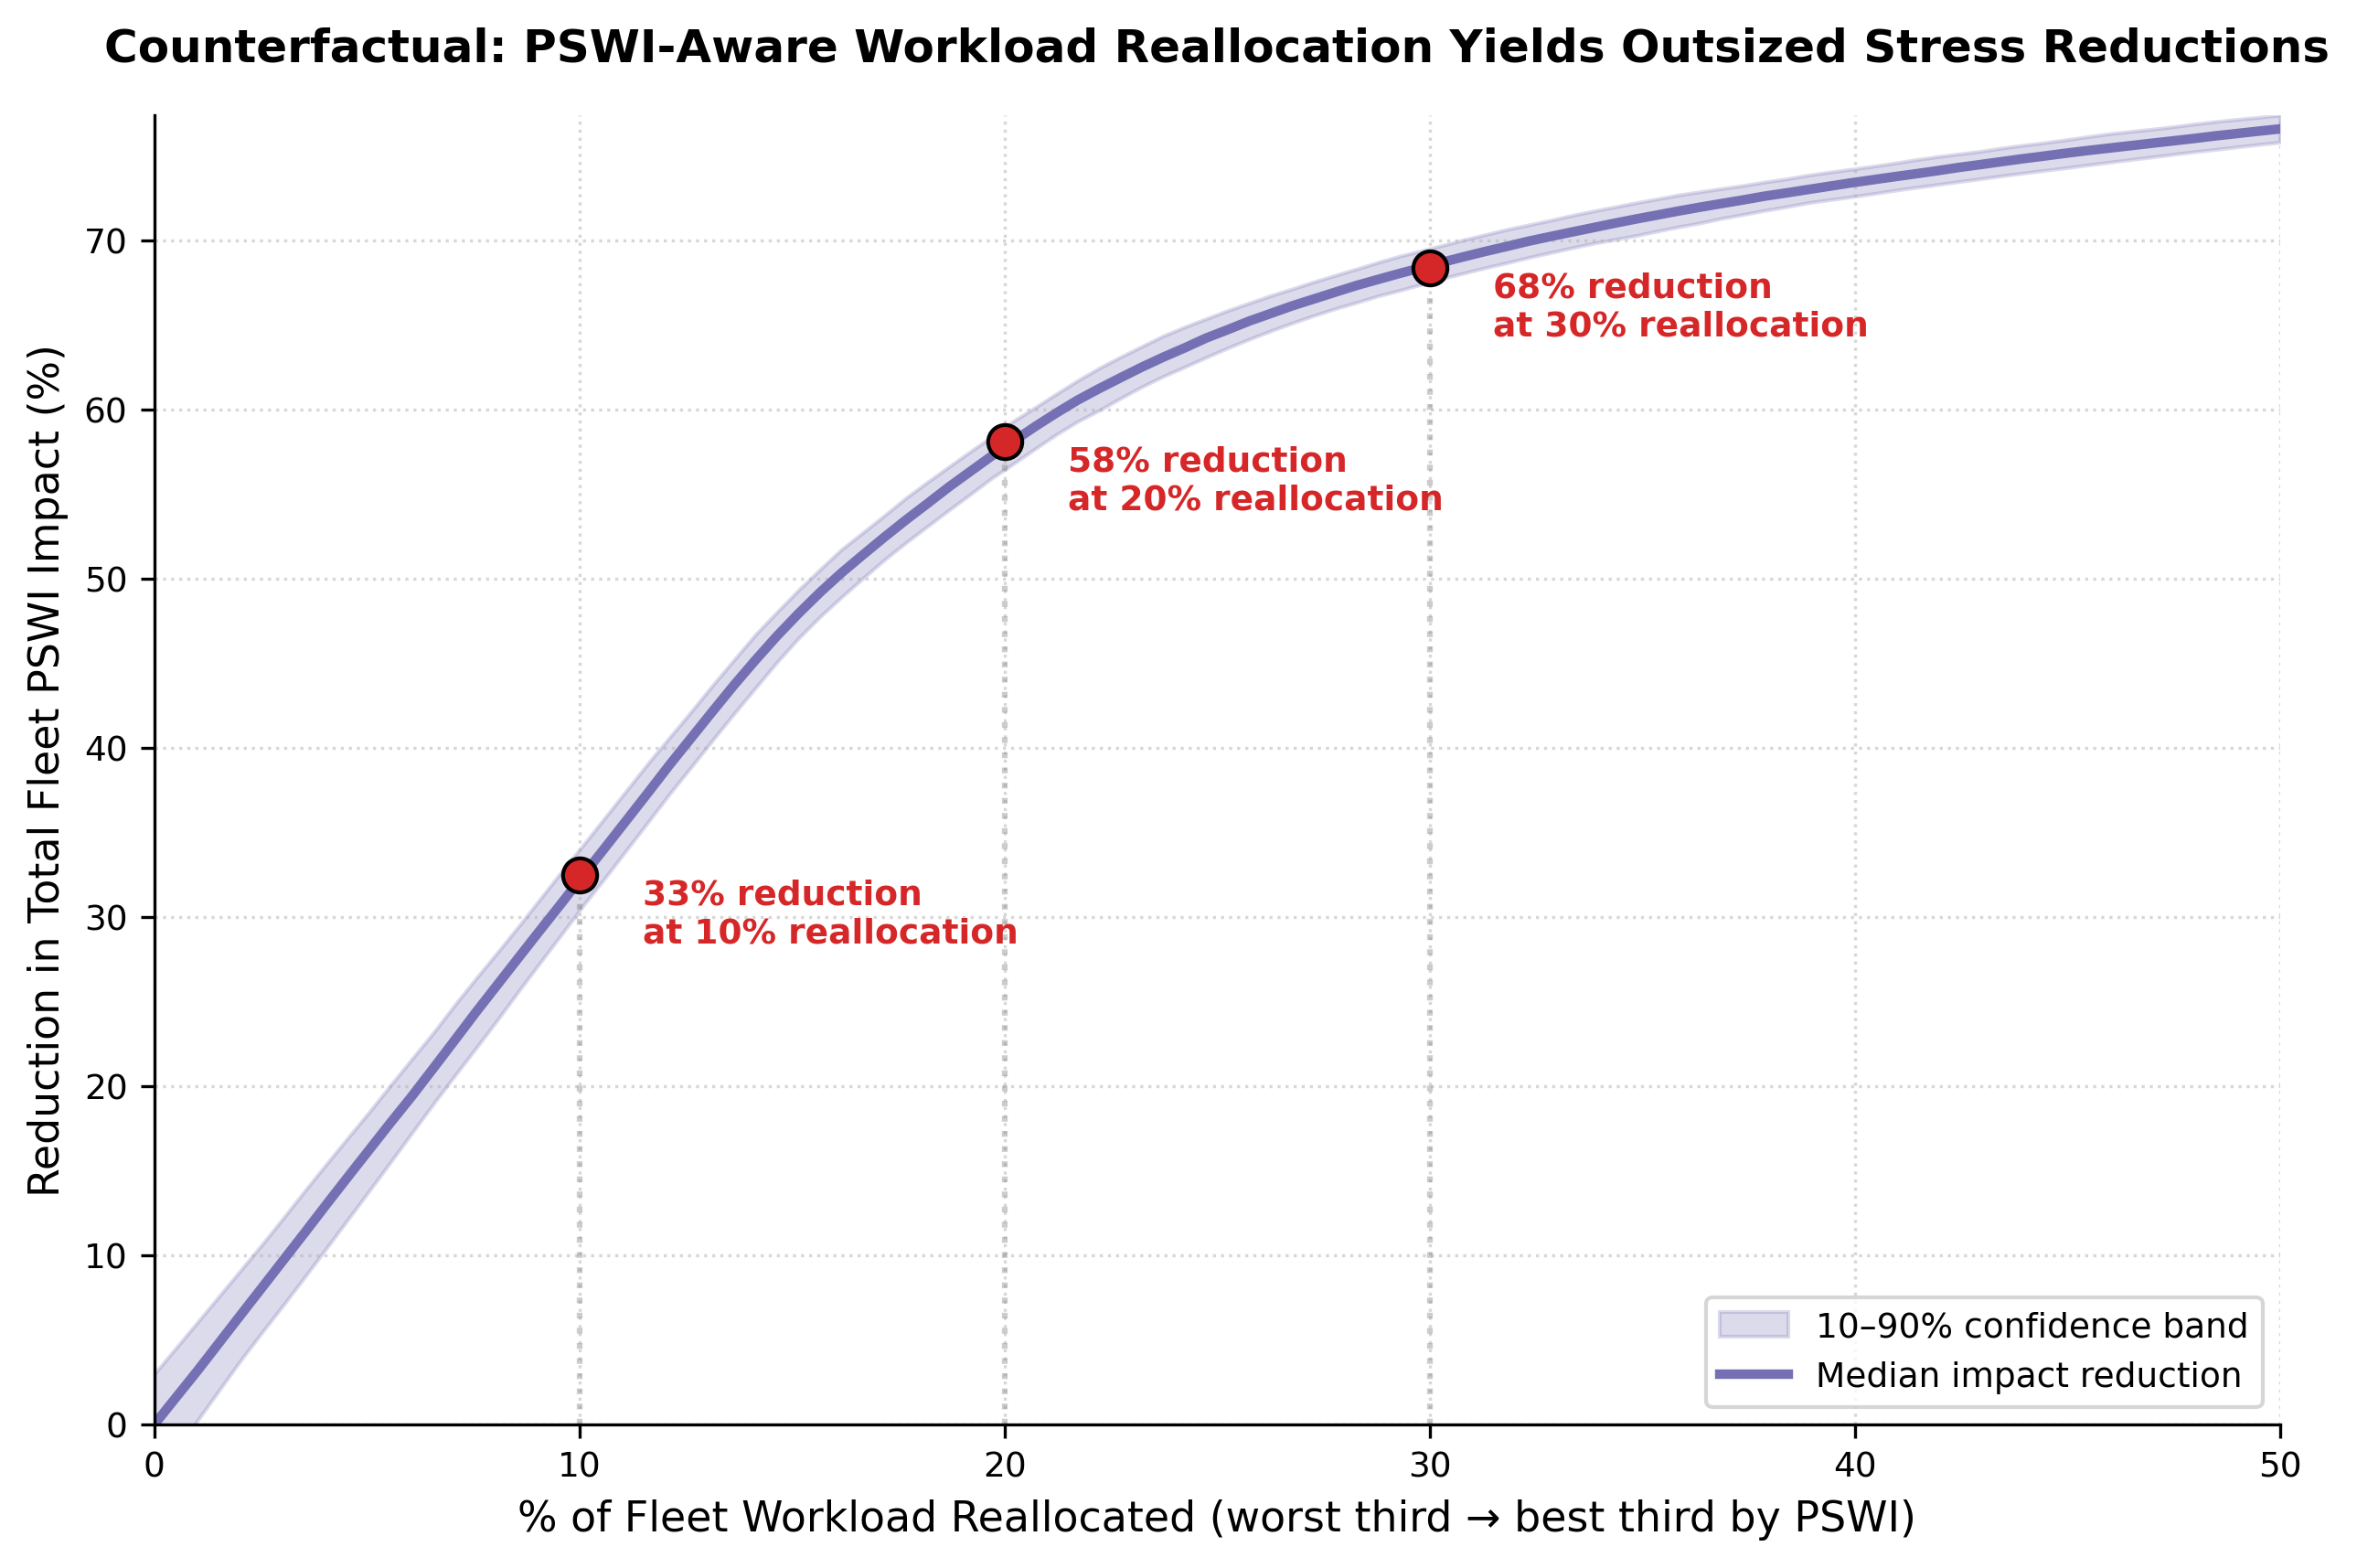
\includegraphics[width=\columnwidth]{../figures/figure_5_counterfactual.png}
\caption{Counterfactual impact reduction under PSWI-aware workload
reallocation. Reallocating just 10\% of fleet workload from the
worst-PSWI third to the best-PSWI third yields a 33\% reduction in
total fleet water-stress impact.}
\label{fig:counterfactual}
\end{figure}

\paragraph{Interpretation.}
The concavity of the curve is the policy-relevant finding. It implies
that a regulator or operator does not need to mandate large workload
shifts to achieve substantial impact reduction; the marginal worst
facilities account for a disproportionate share of total fleet impact.
This is the same reasoning that motivates progressive carbon pricing
and is structurally analogous: in both cases, a long right tail of
high-impact emitters dominates the aggregate, and targeting the tail
is more efficient than uniform mitigation.

\subsection{Proposed disclosure framework}

We propose a regulatory framework, modeled on the U.S. Securities and
Exchange Commission's Regulation S-K~\cite{secregsk}, that would
require data center operators to publicly report PSWI on a
per-facility, per-quarter basis. Three core requirements are:

\begin{enumerate}
    \item \textbf{Per-facility WUE.} Operators must report annualized
        WUE for each individual facility, identified by physical
        address and operating subsidiary. Aggregation across
        facilities is not permitted.
    \item \textbf{Peak monthly WUE.} Operators must report monthly WUE
        for each facility, enabling computation of a 12-month rolling
        peak as the basis for $\beta$.
    \item \textbf{Source-resolved water inputs.} Operators must
        distinguish potable from non-potable water and report
        withdrawal and consumption separately, with attribution to
        the public water system or alternative source.
\end{enumerate}

A regulator (e.g., the EPA in the U.S., or DG Environment in the EU)
would then publish a quarterly PSWI ranking using these inputs and
WRI Aqueduct's most recent annual dataset, and water utilities would
have standing to challenge new data center siting in catchments with
$\textrm{BWS} > 1$ where the proposed facility's projected PSWI
exceeds 5.

\subsection{Enforcement leverage}

A novel feature of our proposal is that enforcement does not require
new statutory authority. U.S. public water systems already have
permitting authority over large water users under the Safe Drinking
Water Act and state-level analogs~\cite{epa2024watercongress}. The
proposal here is to require PSWI disclosure as a condition of
permitting, leveraging existing utility authority rather than creating
new federal mandates. This pragmatic approach has parallels in
financial regulation: the SEC requires specific disclosures as a
condition of market access, rather than directly regulating issuer
behavior.

% =============================================================================
\section{Limitations and Future Work}
\label{sec:limitations}
% =============================================================================

We document our limitations transparently to support principled
critique and future extension.

\paragraph{Peaking factor estimation.}
We estimate $\beta$ by climate zone, not measurement. This is a
deliberately conservative choice: our climate-zone defaults are at or
below the lower end of Han et al.'s~\cite{han2026} observed range. A
future revision will use disclosed monthly water consumption (currently
available only from Google~\cite{google2025envreport}) or estimates
based on cooling-degree-day patterns at hourly resolution.

\paragraph{Annual BWS averaging.}
We use Aqueduct's annual BWS values, which average across seasons.
Aqueduct also publishes monthly BWS data~\cite{kuzma2023aqueduct},
which would refine the metric: a facility may have moderate annual
stress but extreme summer stress, and PSWI's policy relevance is
greatest in those summer months. Integration of monthly BWS is the
single highest-priority future extension of this work.

\paragraph{Scope 2 omission.}
Like Han et al.~\cite{han2026}, we focus on direct (Scope~1) water use
because it predominantly draws from public water systems. Scope 2
water associated with electricity generation is substantial but draws
mostly from non-potable sources~\cite{li2023thirsty}. A holistic water
sustainability metric should eventually integrate both.

\paragraph{Disclosure-driven coverage bias.}
Our coverage skews toward operators that disclose more data. We have
zero coverage of Chinese hyperscalers (Alibaba, Tencent, Baidu) and
limited coverage of emerging operators in the Middle East and India,
where data center construction is accelerating but disclosure is
nascent. The dataset will expand as global disclosure norms evolve.

\paragraph{No causal claim.}
We do not claim that PSWI \emph{causes} specific water-system harms.
Our claim is narrower: PSWI captures information that is policy-relevant
and currently invisible in disclosed data. Empirical validation against
observed water-system stress events is a natural follow-up study.

% =============================================================================
\section{Conclusion}
\label{sec:conclusion}
% =============================================================================

The water sustainability of AI data centers is shaped by two factors
that current industry metrics conceal: the temporal concentration of
demand on peak summer days, and the spatial heterogeneity of water
stress at facility locations. We have introduced the Peak-Stress Water
Index (PSWI) as a composite metric that integrates both, applied it to
the first cross-company global dataset of major data centers, and
documented findings of policy significance: a 4{,}100$\times$ disparity
between best and worst facilities, systematic rank shifts between
WUE-based and PSWI-based comparisons, and a counterfactual showing
that modest workload reallocation could yield outsized stress
reductions. We have proposed a regulatory framework requiring
per-facility, per-quarter PSWI disclosure, modeled on existing
financial-disclosure architecture and leveraging existing utility
permitting authority. All data and code are publicly released to
enable independent verification and policy adoption. As the AI buildout
continues at projected double-digit annual growth rates, the structural
deficiencies of WUE will become increasingly costly. PSWI is a tractable
step toward a sustainability metric that makes the hidden currents of
data center water use visible to the communities they affect.

% =============================================================================
\section*{Acknowledgments}
% =============================================================================

The author thanks the authors of Han et al.~(2026), Wu et al.~(2025),
and Li et al.~(2024, 2025) for foundational work that made this
synthesis possible. The World Resources Institute provided the
Aqueduct 4.0 dataset under a Creative Commons license, without which
location-specific stress weighting would not have been feasible.

% =============================================================================
% References
% =============================================================================

\bibliographystyle{IEEEtran}
\bibliography{references}

\end{document}
